\section{Related Work}\label{rel_work}

\begin{figure}
\centering
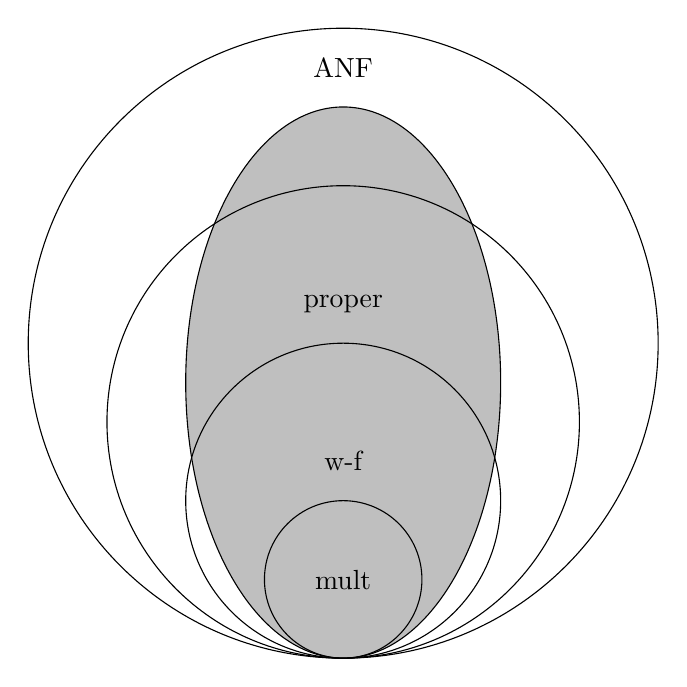
\begin{tikzpicture}
\draw[fill=lightgray](0,-0.5) ellipse (2cm and 3.5cm);
\draw{(0,0) circle(4cm)};
\node at (0,3.5) {ANF};
\draw{(0,-1) circle(3cm)};
\node at (0,0.5) {proper};
\draw{(0,-2) circle(2cm)};
\node at (0,-1.5) {w-f};
\draw{(0,-3) circle(1cm)};
\node at (0,-3) {mult};

\end{tikzpicture}
\caption{Relationships between the sets of constraints where \enquote{w-f} is an abbreviation for well-formedness and \enquote{mult} is an abbreviation for multiplicity.
The set of circular conflict-free constraints is highlighted in grey.}\label{venn}
\end{figure}

In this section, we summarise other approaches for rule-based graph repair and compare them to our approach.
An overview of the relations of all constraint types mentioned below is shown in Figure \ref{venn}. \\ \\
\textbf{Iterative Development of Consistency-Preserving Rule-Based Refactorings}: Becker et al. \cite{becker2011iterative} introduced an interactive approach to construct con\-sis\-tency-\-pre\-ser\-ving transformations based on their invariant checker introduced in \cite{becker2006symbolic} for so-called \emph{well-formedness constraints}. 

These are constraints of the form $\neg \exists (c_1, \true)$ or $\forall (C_1,  \exists(C_2, \true))$.
Given a consistent graph, a well-formedness constraint and a refactoring specification, which is a set of rules in the single-pushout approach \cite{hartmut2006fundamentals}, the invariant checker constructs all minimal counterexamples that lead to a non-consistency preserving transformation via rules of the refactoring specification. If there are no such counterexamples, then any transformation with a rule of the refactoring specification is consistency-preserving.
This approach is designed to be fully interactive, requiring the user to revise the refactoring specification until no counterexamples are returned.

Our approach allows the automatic construction of consistency-preserving rule sets w.r.t. a set of constraints in ANF. The results of section \ref{comp_general} show that every direct consistency-preserving rule is also a consistency-preserving rule, and therefore all rules of a rule set $\mathcal{R}$ can be equipped with the direct consistency-maintaining application condition introduced in section \ref{appl_conds}. This newly created rule set contains only consistency-preserving rules.
\\ \\
\textbf{Ensuring Consistency of Conditional Graph Grammars:} Heckel and Wagner \cite{heckel1995ensuring} have presented an approach to construct consistency-preserving application conditions for rules in the single-pushout approach and  constraints of the form $\forall(C_1, \exists (C'_1, \true)) \wedge \ldots \wedge \forall(C_n, \exists (C'_n, \true))$.
Although the constructed application conditions are not presented as nested conditions, they can be transformed into nested conditions of the form $\forall(C_1, \exists(C_1^1, \true) \vee \ldots \vee \exists(C_1^{k_1}, \true)) \wedge \ldots \wedge \forall(C_n, \exists(C_n^1, \true) \vee \ldots \vee \exists(C_1^{k_n}, \true))$.

Our approach allows the construction of consistency-preserving application conditions for such constraints. A constraint $c$ of the form described above is a conjunction of constraints in UANF. Therefore, we can construct the direct consistency-maintaining application conditions for all these constraints. The conjunction of these application conditions is a direct consistency-maintaining and therefore a consistency-preserving application condition for $c$.
\\ \\
\textbf{Sustaining and Improving graduated Graph Consistency}:
Kosiol et al. \cite{kosiol2022sustaining} have introduced the notions of (direct) consistency-sustaining and (direct) consistency-improving transformations as already introduced in section \ref{sec_consistency}.
This approach is designed for rules in the double-pushout approach and nested conditions in ANF. 
They have introduced a method for constructing consistency-sustaining application conditions, a sufficient criterion for consistency-sustaining  transformations and a necessary criterion for consistency-improving transformations. Both criteria have been implemented and evaluated. 


As already discussed, our notions of (direct) consistency-maintaining and (direct) consistency-increasing application conditions are more fine grained and in generally not related to those described in \cite{kosiol2022sustaining}. 
If the nesting level of a constraint $c$ is $1$, these notions are identical and any consistency-increasing application condition at layer $-1$ for $c$ is also a consistency-increasing application condition for $c$. 
Therefore, a consistency-increasing application condition at layer $-1$ for $c$ is also consistency-improving application condition for $c$.

Any consistency-maintaining application condition constructed by Theorem \ref{appl-main} contains a consistency-sustaining application condition constructed by the approach of \cite{kosiol2022sustaining}. Therefore, these consistency-maintaining application conditions are also consistency-sustaining ones. However, because these consistency-maintaining application conditions also contain additional conditions, a con\-sis\-ten\-cy-maintaining application condition is more restrictive and complex than a application condition constructed using the method introduced in \cite{kosiol2022sustaining}. 
\\ \\
\textbf{Constructing optimized constraint-preserving application conditions for mo\-del transformation rules}:
Nassar et al. \cite{nassar2020constructing} have introduced a method for constructing consistency-sustaining and consistency-preserving application conditions in the framework of $\mathcal{M}-$adhesive categories.
Due to some optimisations, these application conditions are less restrictive and less complex than those described in \cite{habel2009correctness} and \cite{kosiol2022sustaining}. They have introduced the notion of \emph{weakest application conditions}.
As the name suggests, a weakest application condition is implied by any other application condition with the same property. 
For example, a weakest consistency-preserving application condition is implied by every other consistency-preserving application condition. The construction of the application conditions has been implemented as an eclipse plug-in called \emph{OCL2AC}, which is able to construct consistency-guaranteeing, weakest consistency-preserving or consistency-sustaining application conditions.

Some of the optimisations presented could also be used to optimise the application conditions we have introduced. 
In particular, these optimisations could be used to reduce the complexity of the direct consistency-maintaining and consistency-increasing application conditions at layer for general rules. 
We have already indicated that the application conditions introduced in Section \ref{appl_conds} are not weakest conditions, 
and that constructing such weakest direct consistency-maintaining or direct consistency-increasing application conditions would probably lead to huge application conditions.
\\ \\
\textbf{Rule-based Graph Repair}:
Sandmann and Habel \cite{sandmann2019rule} have introduced a repair process for so-called \emph{proper constraints} based on so-called \emph{repair programs}. 
A constraint in ANF is called \emph{proper} if it ends with $\exists(C, \true)$ or is of the form $\exists(C_1, \forall(C_2, \false))$ or $\forall(C_1, \false)$.
The authors describe a method for inductively constructing a repair program consisting of rules in the double-pushout approach that, when applied to a non-consistent graph, returns a consistent graph. 
They have also introduced a graph repair approach given a set of rules $\mathcal{R}$. 
The approach described above can be used to repair a graph with rules from $\mathcal{R}$ if there is a repair program such that for every rule in the repair program there is an equivalent rule in $\mathcal{R}$.

Our approach can repair circular conflict-free constraints. The set of circular conflict-free constraints and the set of proper constraints intersect, but the set of circular conflict-free constraints is not contained in the set of proper constraints. Note that a constraint $c$ in ANF is not proper if it ends with $\forall(C_{\nlvl(c)}, \false)$ and $\nlvl(c) > 2$. Therefore, a non-proper circular conflict-free constraint can be easily constructed. 
Furthermore, our approach can repair a set $\mathcal{C}$ of circular conflict-free constraints, if $\mathcal{C}$ is a circular conflict-free set of constraints w.r.t. to a rule set $\mathcal{R}$ and $\mathcal{R}$ is a repairing set for $\mathcal{C}$. 
\\ \\
\textbf{Rule-based Repair of EMF Models}:
Nassar et al. \cite{nassar2017rule, nassar2017rule1} have introduced a repair approach for models of the \emph{eclipse modeling framework} (EMF) \cite{steinberg2008emf}. In particular, this approach is able to repair multiplicities of a given EMF metamodel. 
Multiplicities can be described as nested conditions of the form $\forall(C_1, \exists(C_2, \true))$ and $\forall(C_1, \false)$. 
The approach was implemented using two Eclipse plugins in Henshin \cite{arendt2010henshin}. One plugin derives rules for the repair process from a metamodel. The other plugin is an implementation of the repairing process.

Every upper bound of a multiplicity can be described as a constraint of the form $\forall(C_1, \true)$. Such a constraint is always circular conflict-free. In addition, a lower bound of a multiplicity can be described as a constraint of the form $\forall(C_1, \exists(C_2, \true))$ where $C_1$ contains exactly one node and no edges. Therefore, such a constraint is also always circular conflict-free. 
This implies, that our approach can repair a set of multiplicities, if an appropriate set of rules $\mathcal{R}$ is used. That is, the set of multiplicities is a circular conflict-free set of constraints w.r.t. $\mathcal{R}$, and $\mathcal{R}$ is a repairing set for $\mathcal{C}$.
